\documentclass[a4paper, 10pt, conference]{ieeeconf}


%%%%%%%%%%%%
% Packages %
%%%%%%%%%%%%

\usepackage[utf8]{inputenc}
\usepackage[T1]{fontenc}

\usepackage{amsmath}
\usepackage{amssymb}

\usepackage{graphicx}
\usepackage{hyperref}
\usepackage{tabularx}

\usepackage{cite}

\usepackage{layout}
\usepackage{lipsum}

\usepackage{siunitx}

\usepackage{caption}
\usepackage{subcaption}


%%%%%%%%%%%%%%%%%%
% Configurations %
%%%%%%%%%%%%%%%%%%

\makeatletter
\def\title#1{\gdef\@title{\LARGE\bfseries#1}}
\makeatother
\setlength{\topmargin}{0pt}
\setlength{\oddsidemargin}{-18pt}

\title{INFO0948-1: Final report}
\author{Maxime \textsc{Meurisse} (s161278) \and Valentin \textsc{Vermeylen} (s162864)}


%%%%%%%%%%%%
% Document %
%%%%%%%%%%%%

\begin{document}
    % ----- Title page ----- %
    
    \maketitle
    \thispagestyle{plain}
    \pagestyle{plain}
    
    % ----- Introduction ----- %
    
    \section{Introduction}
    
    The goal of this project was to learn how to manipulate a robot (a \emph{youBot} from \href{https://www.kuka.com/}{KUKA}) equipped with some sensors (Hokuyo and RGBD), represented in Fig. \ref{fig:introduction.youbot}, in order to automate simple tasks.
    
    \begin{figure}[!h]
        \centering
        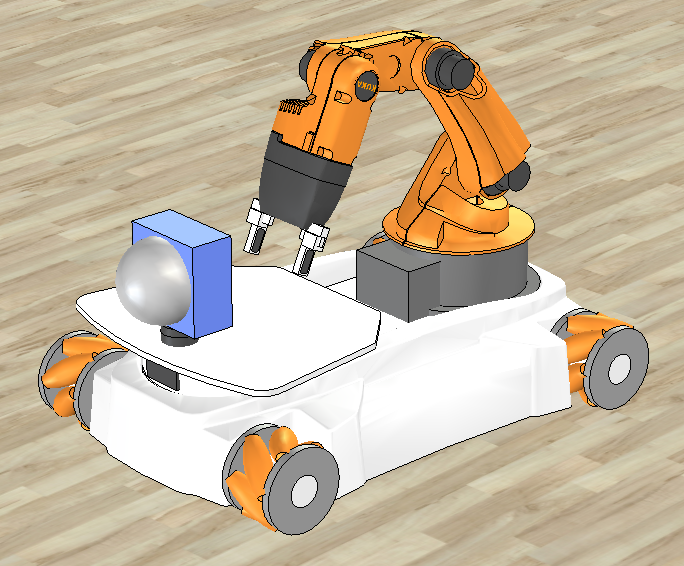
\includegraphics[width=0.25\textwidth]{resources/png/youbot.png}
        \caption{The youBot robot used for the project.}
        \label{fig:introduction.youbot}
    \end{figure}
    
    The first step was to navigate in an unknown environment (but of known dimensions) to produce a precise representation that could be used later (typically a two-dimensional map). This task, which we will call "navigation" later on, is fully explained in section \ref{sec:navigation}.
    
    An example environment for the robot is shown in Fig. \ref{fig:introduction.environment}.
    
    \begin{figure}[!h]
        \centering
        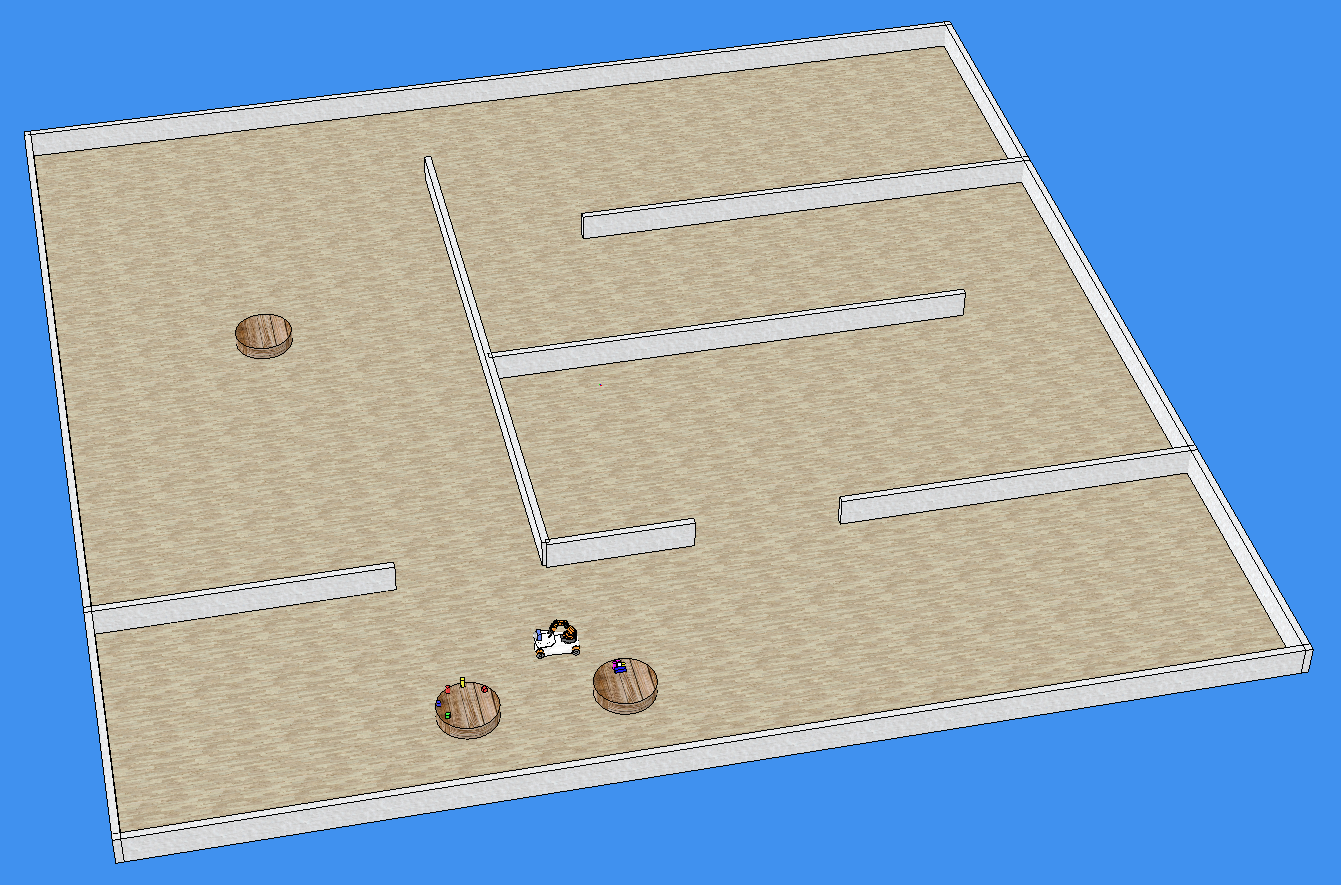
\includegraphics[width=0.25\textwidth]{resources/png/environment.png}
        \caption{An example of environment for the robot.}
        \label{fig:introduction.environment}
    \end{figure}
    
    The second step consisted of transporting, using the robot arm, objects from one table to another. This task, which we will call "manipulation" later, is fully explained in section \ref{sec:manipulation}.
    
    Both tasks must be performed completely autonomously by the robot, regardless of the environment in which it is located. No human intervention shall be necessary.
    
    To carry out this project, we used the V-REP simulator (from \href{https://www.coppeliarobotics.com}{Coppelia Robotics}) to simulate the youBot and its environment. We used the MATLAB language and several of its toolboxes to program and plan the robot's actions.
    
    Our implementation allowed the youBot to successfully perform navigation and manipulation. A video showing the robot in action is available via the following link:
    
    \begin{center}
        \href{to do}{to do}
    \end{center}
    
    This document will begin by briefly explaining the organization of the code. Then, it will explain in a general way, via a diagram representing the finite state machine, how the robot plans its actions. Each milestone (navigation and manipulation) will then be detailed: strategy used, problems encountered, etc. Finally, this document will end with possible improvements to our implementation and a conclusion.
    
    % ----- Code organization ----- %
    
    \section{Code organization}
    
    We have chosen to work mainly with the \emph{object-oriented} paradigm. We have therefore identified the main elements and implemented them through objects:
    
    \begin{itemize}
        \item an object \texttt{MapManager} to handle the representation of the environment;
        \item an object \texttt{RobotController} to handle the robot.
    \end{itemize}
    
    Our code is organized like this:
    
    \begin{itemize}
        \item a folder \texttt{classes/} that contains files \texttt{MapManager.m} and \texttt{RobotController.m} mentioned above;
        \item a folder \texttt{imported/} that contains all the functions we found on the Internet. The source of each function is mentioned in the comments of the file;
        \item a folder \texttt{mat/} that contains representations of the environments the robot has explored (in the form of exported MATLAB variables so that they can be saved and reloaded later) and other resources;
        \item a file \texttt{main.m} which is the main file of our implementation;
        \item a file \texttt{manipulation.m} that contains the implementation of the "manipulation" task;
        \item a file \texttt{navigation.m} that contains the implementation of the "navigation" task;
        \item a file \texttt{startup.m} to prepare MATLAB for simulation.
    \end{itemize}
    
    To run the code, first configure the \texttt{trs/} folder (as explained on \href{http://ulgrobotics.github.io/trs/setup.html#install}{the official project website}) and attach it to the code. Then, run the \texttt{startup.m} file (by default, MATLAB should run it automatically at startup). Finally, just run the \texttt{main.m} file. The latter can be edited to change the dimensions of the map, the time in seconds between two scans correction, and other parameters.
    
    We have tried to make our code as simple, readable, and understandable as possible. We have exploited the object-oriented paradigm to avoid code repetition and to encapsulate the actions of each element neatly. So we have a very simplified interface for the robot and the map (e.g. \texttt{robot.move(objective)} to move the robot to the objective \texttt{objective}, \texttt{map.show()} to display the map, etc), which greatly simplifies our life afterwards for the use and maintainability of the code.
    
    % ----- Finite state machine ----- %
    
    \section{Finite state machine}
    
    In order to accomplish both tasks, the robot performs a series of actions in a specific order. All these actions are summarized in the finite state machine shown in Fig. \ref{fig:fsm}\footnote{The figure is in vectorial format, do not hesitate to zoom in on it for better visibility.}, in the appendix.
    
    The robot states for navigation are implemented in the \texttt{navigation.m} file. The robot states for manipulation are implemented in the \texttt{manipulation.m} file.
    
    Since the simulator works with a \SI{50}{\milli\second} time step, the main difficulty is to make each action of the finite state machine execute within \SI{50}{\milli\second}. We have optimized our coding as much as possible and, in general, it runs well under this constraint. Only the actions like the movements of the robot arm take more time. For the latter, we stop the robot to avoid inconsistencies in its movements due to the time lag with the simulator.
    
    We noticed that the rendering of the map took a lot of time (about \SI{20}{\milli\second} for navigation and about \SI{40}{\milli\second} for manipulation). So we decided to update the map only every \num{50} iterations for navigation. Concerning the manipulation, we believe that the map, not evolving over time, is no longer necessary. We are therefore no longer refreshing it (except for few rare exceptions).
    
    % ----- Navigation ----- %
    
    \section{Navigation}\label{sec:navigation}
    
    As shown in the finite state machine (Fig. \ref{fig:fsm}), the robot performs a series of actions to successfully navigate. These series of actions are very similar for each difficulty (milestones 1a, 1b and 1c). Only the action "update position and orientation" varies between the different difficulties.
    
    Each of the actions will be detailed to explain how it works and to justify our choices of implementation.
    
    \subsection{Initialization}
    
    The initialization phase consists of determining the initial position and orientation of the robot. When we have access to the different sensors, we simply use them. When we don't have access to the sensors, we set ourselves an initial position and an initial orientation for the robot (in our case, we decided that the robot starts in the center of the map). Even if this position does not correspond to the real position of the robot (the one returned by its sensors), it does not matter: we build the representation of the map only based on the movements made by the robot; it will be built entirely with respect to the initial position set.
    
    As we do not know where the robot starts, but we know the dimensions of the environment (15 meters by 15 meters), we have created a representation that is twice as long and wide as the size of the environment. This avoids getting negative positions, which is annoying when working with matrices. When we don't have access to the sensors, we therefore set the robot to start at the center of the environment representation, i.e. at point \texttt{[15, 15]}.
    
    When the initial position and orientation are set, we mark the robot's neighborhood as free positions. Indeed, the position of the robot represents a single point on the map, but the robot itself counts for several points since it has a width and a length. In order to take into account all the points that the robot represents, we take into account its neighborhood.
    
    \subsection{Update position and orientation}
    
    This step, and all subsequent steps, are repeated at each iteration. Updating the position and orientation of the robot is done differently depending on the difficulty.
    
    \subsubsection{Permanent access to sensors}
    
    When we have constant access to sensors, we simply use the robot's GPS to update its position and orientation. This operation is very simple and instantaneous.
    
    \subsubsection{Odometry and GPS correction}
    
    For the second navigation milestone, we only have access to the GPS data every minute. The approach we have thus taken is to estimate the position and orientation of the robot at each time step via the odometry. When looking at the function \texttt{youbot\_drive}, we have seen that the angular displacements and rotation between two-time steps can easily be retrieved via a linear combination of the movement of each wheel. Multiplying these values by the radius of the wheels of the robot (\SI{5}{\centi\meter} for the displacements and an experimental value of about \SI{12.75}{\centi\meter} for the rotation), we can get the linear displacements and the rotation in radian.
    
    Plugging these values in the following equations, taken from \textbf{ref} ($v$ is the forward velocity during the time step and $w$ the rotational one),

    \begin{equation*}
        \left(\begin{array}{l}
            x^{\prime} \\ y^{\prime} \\ \theta^{\prime}
        \end{array}\right)
        =
        \left(\begin{array}{l}
            x \\ y \\ \theta
        \end{array}\right)
        +
        \left(\begin{array}{c}
            -\frac{\hat{v}}{\omega} \sin \theta+\frac{\hat{v}}{\omega} \sin (\theta+\hat{\omega} \Delta t) \\ \frac{\hat{\omega}}{\omega} \cos \theta-\frac{\hat{\omega}}{\hat{\omega}} \cos (\theta+\hat{\omega} \Delta t) \\ \hat{\omega} \Delta t
        \end{array}\right)
    \end{equation*}

    we retrieve correct approximations of the displacement of the youBot along both axes. The estimation of the $w$ based on the odometry, however, is far from perfect. Indeed, the relationship that exists between the linear combination of the angular movement of the wheels and the real rotation is semi-linear, but with high variance for small angles, as can be seen in the graph \textbf{mettre graphe ici}. 
    
    Since we have access to the real orientation at all times, it is actually not necessary to estimate the orientation based on the odometry, but it was done in the hope we would get a working SLAM.
    
    Talk about the correction phase.
    
    \subsection{Update data from Hokuyo}
    
    This stage consists in recovering the various points captured by the Hokuyo. We differentiate between free points and contact points and then transform them into absolute coordinates to insert them in our representation of the environment (by default, the points are in coordinates relative to the robot).
    
    The transformation of all the points of the Hokuyo is quite expensive. We used a function, found on the Internet, which simplifies the polygon formed by these points in order to accelerate the process considerably while preserving the appearance of the polygon.
    
    The free points are inserted as such in our map, and the contact points are inserted as walls in our map. It is therefore this step that updates our representation of the environment.
    
    Our implementation, and especially the coordinate transformation, is strongly based on the one given as an example on the \href{https://github.com/ULgRobotics/trs}{GitHub of the course}.
    
    When we don't have access to GPS constantly, we save the different data from the Hokuyo at each iteration in order to correct them later.
    
    \subsection{Obstacle nearby}
    
    When the robot is moving, it can sometimes move towards an obstacle without knowing it (because initially, this obstacle was not yet discovered on the map). To prevent the robot from rushing into it, we have implemented a mechanism that allows it to stop and start again.
    
    To know if an obstacle is near (and in front of) the robot, we select several frontal rays of the Hokuyo and calculate the distances between the robot and the contact points of these rays. If only one of these distances is less than a threshold (which we have set at \SI{50}{\centi\meter} from the center of the robot), we immediately stop the robot. We reset his objective so that he determines a new one and starts again correctly.
    
    When an obstacle has been detected, we no longer perform the check for \num{50} iterations to allow time for the robot to move. Indeed, if the robot is close to an obstacle, it would constantly be considered as such if we check at each iteration and would therefore remain blocked for an infinite time (since it would stop at each iteration and would not have the time to move).
    
    \subsection{Objectives and path finding}
    
    To move the robot, we use a goal and path system. We can distinguish two types of objectives: the current objective and the final objective. The current objective is the next point to which the robot must go. The final objective is the endpoint to which the robot must go.
    
    So the first time we calculate a final objective for the robot. The latter is simply the closest unexplored point of the robot on the map. In order to avoid choosing unreachable points, we check that the found point is surrounded by at least one free (thus reachable) point. When this point is determined, we calculate a path to it using the A* algorithm. Once the path is obtained, we determine the robot's next point, its current objective, by simply taking the first point of the path (and removing it from it).
    
    In the next iterations, we check on the robot has a current target. If it does, then we don't do anything more, we let the robot go there. If the robot no longer has a current objective, we choose a new one by taking the first point of the path. And if the path is empty, i.e. the robot has reached its final goal, we recalculate a new next point to explore, and the cycle starts again.
    
    We consider the navigation is finished when no new point to explore can be determined. Indeed, in this case, it means that all points have been explored. We had the initial idea to use, in addition to this technique, a percentage of exploration: we would stop the navigation when the robot had explored more than 99.5\% of the environment. However, due to numerical errors, especially when we don't have constant access to the sensors, this percentage was distorted and exceeded 100\%. So we dropped the idea.
    
    To plan a path, we used the A* algorithm. We found a MATLAB implementation on the Internet and used it. The choice of this algorithm came naturally to us because we had studied it before and its performance is very good. Indeed, it operates under \SI{50}{\milli\second}, which respects the constraint of this project.
    
    However, we have that its execution time is proportional to the size of the environment. To overcome this problem, we thought of using a solution where we define key points on the map, and that we plan a path while still passing these key points. This would drastically reduce the execution time since the algorithm would only act on a few points instead of the whole map. However, with such a solution, the definition of the key points is crucial: if the choice of key points is wrong, the robot may not find a path. So we finally dropped this method to keep the traditional A* algorithm, but we are well aware that on a much larger map, the \SI{50}{\milli\second} threshold may be crossed. For safety reasons due to this threshold, we stop the robot when calling the algorithm.
    
    We also tested the D* algorithm provided with P. Corke's Robotics toolbox, but it was too slow so we dropped it.
    
    \subsection{Move the robot}
    
    To make the robot move, we use its forward-backward and rotational velocities. In order to make the movement smooth, we make the robot move forward and turn at the same time. The challenge is therefore to choose good values for these velocities.
    
    The first step we do is calculate the angle (in an absolute frame of reference) that the robot must have to be aligned with its objective. We then calculate the distance between this angle and the current angle of the robot (the third Euler angle of the robot). We also calculate the distance (L1 norm) between the robot's position and its objective.
    
    The second step is to assign values to the velocities. We distinguish several cases depending on the distance between the angles. If the latter is very high, the robot rotates and does not move forward. If the latter is moderately high, the robot turns and begins to move slowly. If, finally, the distance between the angles is very small, the robot moves forward and does not turn. This fairly simple system makes movement fluid and ensures that the robot does not deviate from its path.
    
    \subsection{Navigation finished}
    
    When the navigation is finished, we obtain a representation of the environment where the free (accessible) points are represented in green and the inaccessible points (walls, tables, etc.) are represented in red.
    
    When GPS is used at each iteration, the representation of the environment is very good and very precise (Fig. \ref{fig:navigation.map.gps}). When the GPS is not used (or only a few times), the representation is inevitably less precise, but quite usable for the future (Fig. \ref{fig:navigation.map.nogps}).
    
    \begin{figure}[!h]
        \centering
        \begin{subfigure}[b]{0.23\textwidth}
            \centering
            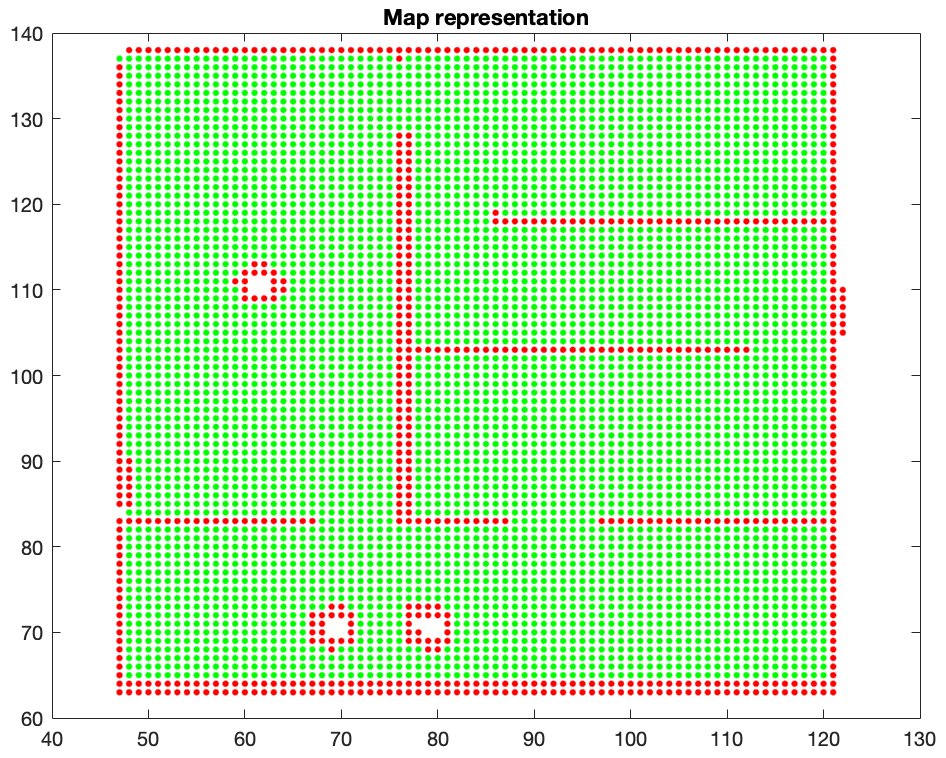
\includegraphics[width=\textwidth]{resources/png/map-gps.png}
            \caption{With GPS.}
            \label{fig:navigation.map.gps}
        \end{subfigure}
        \hfill
        \begin{subfigure}[b]{0.23\textwidth}
            \centering
            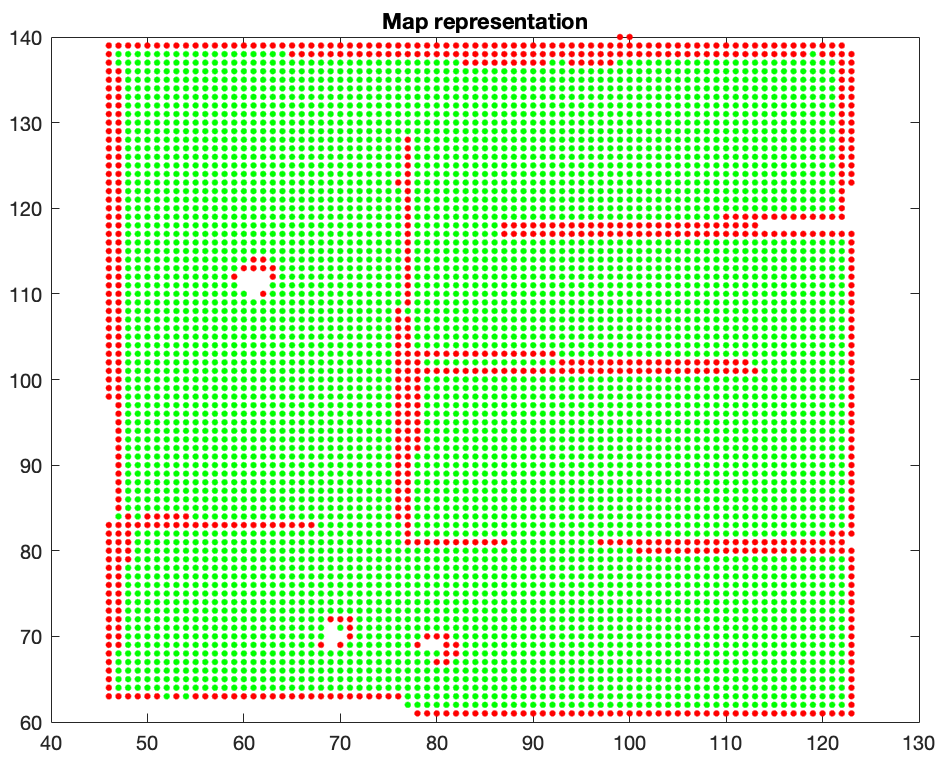
\includegraphics[width=\textwidth]{resources/png/map-nogps.png}
            \caption{Without (or few) GPS.}
            \label{fig:navigation.map.nogps}
        \end{subfigure}
        \caption{Representations of the environment at the end of the navigation.}
        \label{fig:navigation.map}
    \end{figure}
    
    When we have access to the GPS once every minute, we found that waiting for the last update at the end of the navigation allowed us to get a better map for manipulation. So we implemented a mechanism that, when navigation is finished, waits for the last correction with GPS before continuing (so, the robot doesn't move and wait, for a maximum of 1 minute).
    
    % ----- Manipulation ----- %
    
    \section{Manipulation}\label{sec:manipulation}
    
    As illustrated in the finite state machine (Fig. \ref{fig:fsm}), the robot goes through a series of states to perform object manipulation. These states are globally identical for all difficulties. Each state is detailed in the rest of this document.
    
    \subsection{Table detection}
    
    The first step of the manipulation consists in detecting the position of the tables on the map representation obtained with the manipulation.
    
    To do this, we use MATLAB's \texttt{imfindcircles} function. This uses a \emph{circle Hough transform} to detect all the circles on an image. The image considered here is the occupancy matrix corresponding to the obtained occupancy map. This matrix has values of $0$ for free positions and values of $1$ for an occupied position, so it is a binary image.
    
    This function easily finds the circles when the map is accurate. However, if the map is not precise (which is the case when we work with odometry and little GPS), the tables are sometimes represented by a few scattered pixels and therefore not detected by the function.
    
    To overcome this, we did pre-processing on the matrix. First, we make an inflate of it. This allows us to inflate the dot amats. Secondly, we quadruple the resolution of the image. Indeed, by default it is $150\times150$ pixels, and the tables are therefore a few pixels in radius, which is not easy to detect by MATLAB. Finally, we vary the parameters of the \texttt{imfindcircles} function in order to make it more flexible.
    
    When the center of each table is detected, we manually set the radius to \SI{40}{\centi\meter} (because we know that the radius of the tables is \SI{40}{\centi\meter} by checking in the simulator). If we didn't have this data, we would simply have taken the radius values returned by MATLAB.
    
    This detection is quite robust; even if the map representation is approximate, tables are still detected (example in Fig. \ref{fig:manipulation.imfindcircles}).
    
    \begin{figure}[!h]
        \centering
        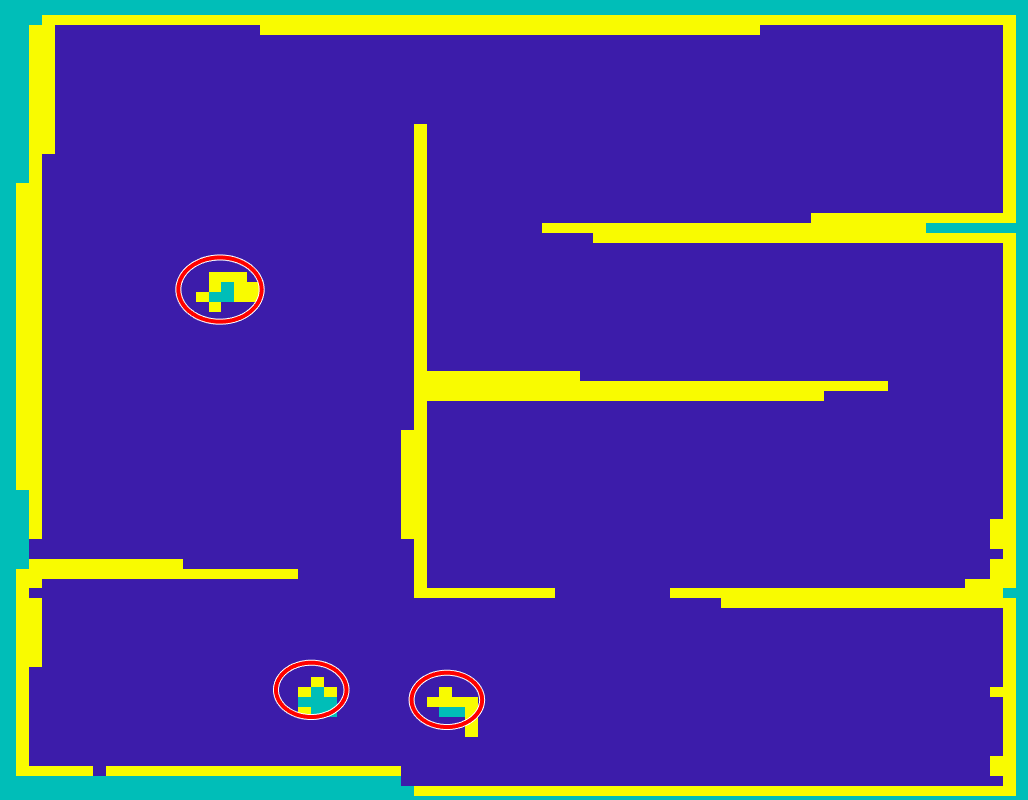
\includegraphics[width=0.3\textwidth]{resources/png/imfindcircles.png}
        \caption{Table detection on an approximate map.}
        \label{fig:manipulation.imfindcircles}
    \end{figure}
    
    If MATLAB cannot find all three tables, we restart a search by varying the parameters and making the search more flexible. Our search is therefore based on the assumption that three tables are present on the map and that each table has a radius of \SI{40}{\centi\meter}. This assumption can be modified in the \texttt{main.m} file of the project. If MATLAB really does not find the circles, we stop the manipulation and display an error message.
    
    \emph{Remark}: we have fixed the assumptions concerning the tables because we are certain, given the project statement, that the tables will always be identical. If we hadn't had the assumptions, our detection would still have worked. We would simply have to filter the detections to be sure that they each correspond to a table (by visiting the place and analyzing it with a 3D point cloud for example).
    
    \subsubsection{Circle Hough transform}
    
    The MATLAB's \texttt{imfindcircles} function allows us to detect circles in an image via a circle Hough transform. This process is similar to the Hough transform, which we studied during the Computer Vision course, which allows lines to be detected. This function therefore works with the equation of a circle rather than the equation of a line.
    
    \subsection{Table exploration and analysis}
    
    The second step consists in exploring each of the detected tables and analyzing it in order to determine its type (empty, easy or hard).
    
    So we start by bringing the robot close to a table (we explore the tables from the closest to the furthest away from the robot). To do this, we generate $15$ points around the table (with a margin of a few centimeters so that the points are far from the table) and we bring the robot to the point that is closest to it. Then we align the robot with the center of the table. Knowing the position of the robot and the position of the center of the table, it is easy to know the angle to be aligned to the table.
    
    When we don't use GPS (or very little), this alignment step is more complex. Indeed, the center of the table and the position of the robot are both based on estimated data and not exact data. To overcome this problem, we make the robot align towards the center of the table using a 3D point cloud: we filter the points to keep only those of the table and we find the closest point to the robot. Then we align the robot facing this closest point.
    
    Then, when the robot is aligned facing the table, we bring it a few centimeters closer (using distances calculated on the basis of Hokuyo) and we take a 3D cloud point (quite large) of the table. We eliminate the points that are too distant and too low so that we keep only the points representing the objects. We then use MATLAB's \texttt{pcsegdist} function to segment the points into different clusters. We set that two points are considered to belong to two different clusters if they are more than \SI{10}{\centi\meter} apart. Thus, on the empty table we get no clusters, on the easy table we get $5$ (or $4$ depending on the viewing angle) clusters, and on the difficult table we get $1$ cluster. We can then easily determine the type of the table according to the number of clusters found.
    
    An example of the clusters obtained is shown in Fig. \ref{fig:manipulation.clusters.easy} and \ref{fig:manipulation.clusters.hard}.
    
    \begin{figure}[!h]
        \centering
        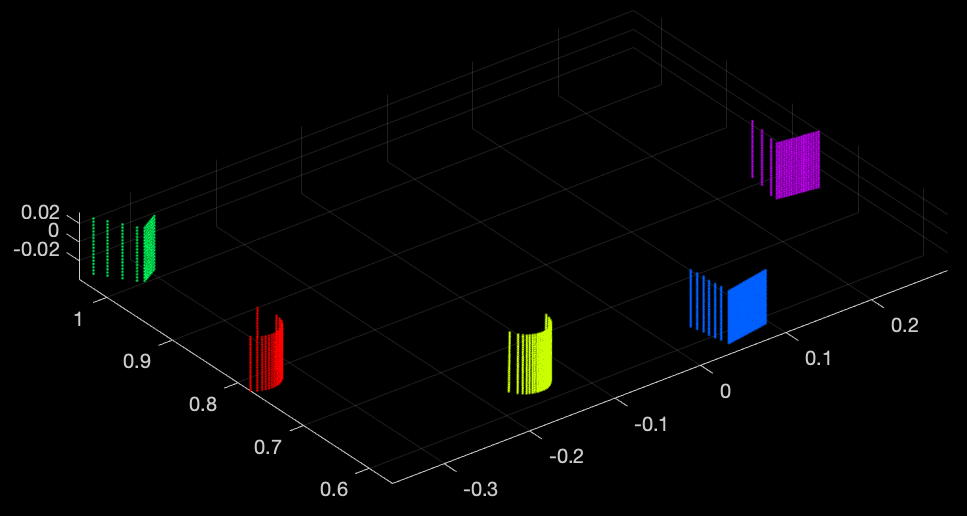
\includegraphics[width=0.4\textwidth]{resources/png/clusters-easy.png}
        \caption{Easy table clusters.}
        \label{fig:manipulation.clusters.easy}
    \end{figure}
    
    \begin{figure}[!h]
        \centering
        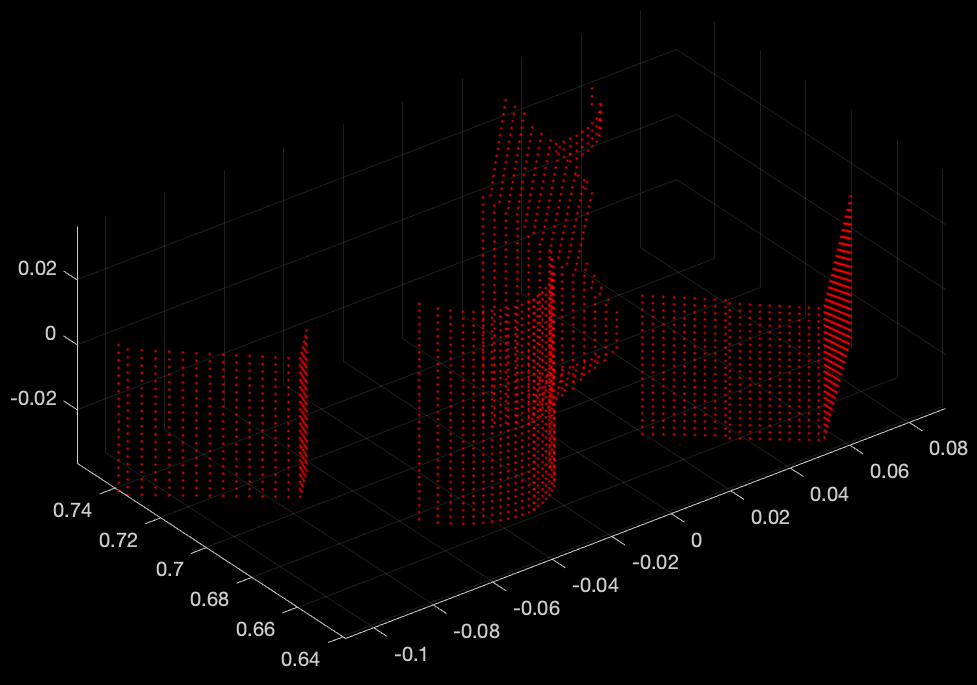
\includegraphics[width=0.4\textwidth]{resources/png/clusters-hard.png}
        \caption{Hard table cluster.}
        \label{fig:manipulation.clusters.hard}
    \end{figure}
    
    The advantage of this method is that it is particularly robust: it does not depend on the color or shape of the objects. Initially, we took a photo and analyzed the colors present in the photo. This technique worked, but was color-dependent, which was not robust.
    
    In order to save time for further manipulation, we already calculate the (central) position of the objects on the basis of these clusters. These positions will be used to grab the objects.
    
    For the difficult table, in order to separate the objects into different clusters, we re-use MATLAB's \texttt{pcsegdist} function, but this time with a smaller distance between each cluster.
    
    To calculate the position of an object, we isolate all the points in its cluster and simply calculate the average position of all the points. These positions are then converted into the absolute coordinate system. Knowing the position and orientation of the robot, the conversion from relative to absolute coordinates is trivial.
    
    \subsubsection{\texttt{pcsegdist} function}
    
    This function of MATLAB allows us to separate the different points of a 3D point cloud from a clustered point. We learned about its operation in order to understand it: the function simply calculates the Euclidean distance from a point to all its neighbors and decides, based on this distance, if the point belongs to the same cluster as its neighbors or if it forms a new cluster. The threshold on the distance is a configurable data.
    
    \subsection{Grabbing an object}
    
    The third step is to grab an object. To do this, we start by making the robot go near the object. We use the same system as before: we generate points around the table and take the point closest to the object (the absolute position of the objects was determined in the previous step). When the robot has reached this point, we align it with the object (same principle as for aligning the robot with the center of the table).
    
    Again, when we do not have access to GPS frequently, relying only on the position of the object to align the robot is not always reliable. In this case, we take a 3D cloud point when the robot is close to the table and align it with the center of the table (with the same 3D cloud point analysis as the previous step). The robot is then aligned with the center of the table and not with the object, but it doesn't really matter.
    
    When the robot is globally aligned with its target, it then moves to the fine-tuning phase. Indeed, to grab an object, we use the arm and the gripper always in the same way and at the same position (example in Fig. \ref{fig:manipulation.grasp.drop.position}). The robot must therefore be positioned well in front of and at a precise distance from the object (\SI{33}{\centi\meter}).
    
    \begin{figure}[!h]
        \centering
        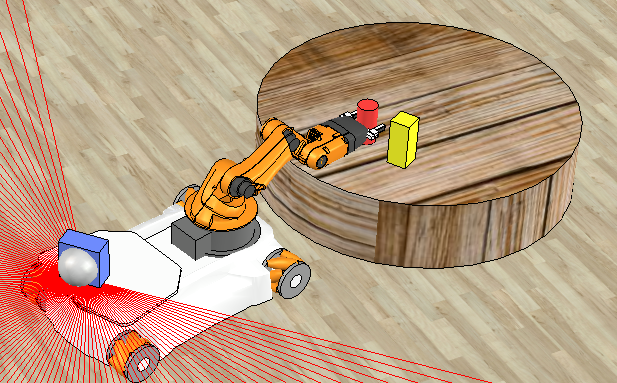
\includegraphics[width=0.4\textwidth]{resources/png/grasp-drop-position.png}
        \caption{Fixed grab and drop position of the robot.}
        \label{fig:manipulation.grasp.drop.position}
    \end{figure}
    
    To align the robot well in front of the object, we take 3D point clouds, isolate the point cluster of the closest object and calculate its central point. According to the x-coordinate of this point, we can tell if the robot is well aligned or not (if $x = 0$, the robot is well in front of the object, otherwise it must slightly turn left or right).
    
    When the robot is perfectly aligned, we must put it at a precise distance from the object. To do this, we take 3D point clouds again and calculate the central point of the closest object. We calculate the distance between this point and the sensor of the robot. According to the found distance, we know if we have to move the robot forward or backward slightly.
    
    Finally, when the robot is well aligned and at the right distance, we make it do a half-turn and grab the object with its arm, always in the same way. When the object is grabbed, we put the arm back to a fixed position so that the object is on the tray, stuck in the gripper.
    
    This technique has the merit of being quite simple and functional. It can however fail because the robot does not necessarily align itself facing one of the faces of the object (if the object is a parallelepiped for example). In this case, the gripper may not grab the object.
    
    This problem occurs very rarely because, even when the robot is not in front of a face, the gripper manages to grab the objects. However, we still implemented a safety mechanism: when the robot grabs (or not) an object, a picture of the gripper is taken. This photo is processed (cropped, reduced and transformed into black and white) and then compared, via a correlation coefficient, to a reference photo of the empty gripper. If the correlation is strong, it means that the gripper is (probably) empty and therefore that the robot has missed its grab. Conversely, if the correlation is low, the grab was successful. When the grab fails, the robot goes back to the position and tries again directly to grab the object.
    
    An example of photos taken and processed is shown in Fig. \ref{fig:manipulation.check.grasp}.
    
    \begin{figure}[!h]
        \centering
        \begin{subfigure}[b]{0.23\textwidth}
            \centering
            
\includegraphics[width=\textwidth]{resources/png/photo-ref.png}
            \caption{Reference photo.}
        \end{subfigure}
        \hfill
        \begin{subfigure}[b]{0.23\textwidth}
            \centering
            
\includegraphics[width=\textwidth]{resources/png/photo-grasp.png}
            \caption{Photo with grasped object.}
        \end{subfigure}
        \caption{Photos taken by the robot to check the grab.}
        \label{fig:manipulation.check.grasp}
    \end{figure}
    
    This mechanism is quite robust and has been proven several times in our simulations.
    
    \subsection{Dropping an object}
    
    The last step is to place the grabbed objects on the objective table.
    
    When the robot has grabbed an object, we start by planning a path to the objective table. To do this, we use the same technique of the previous steps: we generate points around the table and take the closest one to the robot. However, for this step, we try not to take the same one twice so that the robot does not drop two objects in the same place.
    
    When the robot is close to the objective table, we align it with its center. As before, in cases where we have no (or little) access to GPS, we use a 3D point cloud to align the robot.
    
    Once the robot is aligned with the center of the table, we bring it closer to a certain distance (calculated on the basis of the Hokuyo) and make it do a half turn. Finally, he just has to put the object on the table. As for the grab, we use a fixed position of the gripper (see Fig. \ref{fig:manipulation.grasp.drop.position}) to drop the objects.
    
    This technique works very well. In very rare cases, the objects have fallen after being placed on the table. We think that this behavior, a little hazardous, comes from the simulator and not really from our technique. Unfortunately, when the object falls (and rolls off the table), there is not much we can do about it.
    
    \subsection{Manipulation finished}
    
    When the robot has dropped an object, it returns to the table with objects. If it still has object positions in memory, it will face the object and try to grab it. If, on the contrary, it has grabbed all the objects it has spotted during the analysis of the table, it makes a wide 3D cloud point of the table. If it detects objects again, the process starts again. If it doesn't detect any more objects, the manipulation is finished!
    
    In case of a difficult manipulation, the robot does not stop the manipulation but restarts the whole process with the hard table.
    
    Considering the different verifications made (frequent 3D point cloud and pictures were taken), we are almost certain that the robot will grab all the objects and won't forget any of them. Only the drop of the objects is an operation that we cannot verify.
    
    % ----- Retrospective analysis ----- %
    
    \section{Retrospective analysis}
    
    Our implementation has some positive points that we are proud of, but also some negative points that we could improve in the future.
    
    First of all, we are quite satisfied with our code: it is clean, well organized and commented. The object-oriented paradigm allows for clean use and easy maintainability. We are also happy with its robustness: problem situations are, in a majority of cases, detected and handled correctly.
    
    Secondly, we are also happy with the robustness of some of our algorithms: the detection of tables on the map is really reliable, the segmentation of objects in 3D point clouds works quite well and the object grab check mechanism avoids empty round trips between tables.
    
    Concerning the object grasping, our mechanism is not very accurate. Despite our verification system, the robot sometimes grabs objects in an inelegant way. This could have been improved by making a more thorough analysis of the 3D point cloud to determine the position of the faces of the objects and thus be able to align perfectly in front of them.
    
    We are quite happy with our odometry. This seems to work relatively well: we get a representation of the environment that is almost as precise as with GPS. However, in rare cases the representation is poor (some pieces of the wall are forgotten, etc.). We haven't found a robust way to avoid this. But being quite rare cases, we are not too worried.
    
    Finally, regarding pure SLAM, we are disappointed that we did not get there. We tried quite a few techniques, but each time was unsuccessful. We realized that it is not an easy task and that it takes more time than we expected.
    
    % ----- Conclusion ----- %
    
    \section{Conclusion}
    
    This project allowed us to explore a part of the robotics world. Despite the simplifying assumptions, the simple environment and the fairly easy tasks to perform, we realized that it is not easy to create an autonomous robot.
    
    We have learned to use route planning algorithms as well as sensors to discover and analyze an environment as well as to construct a relevant representation of it.
    
    We also learned to manipulate more mechanical aspects of the robot: use of its arm and gripper, precision placement, etc. We made him do simple tasks like grabbing and carrying objects on his own.
    
    All of these tasks have been implemented and completed successfully. Using GPS leads to great results. The use of odometric data leads to less precise results, but quite acceptable and allowing the robot to perform these tasks.
    
    Autonomous control of a robot in a real (simulated) environment is far from easy given the unknown situations and environment. This course allowed us to have the first glimpse of its difficulties and to open the door to the large world of autonomous robots and robotics in general!
    
    % ----- References ----- %
    
    \bibliographystyle{IEEEtran}
    \bibliography{bibfile}
    \nocite{*}
    
    % ----- Finite state machine (figure) ----- %
    
    \newpage
    
    \begin{figure*}
        \centering
        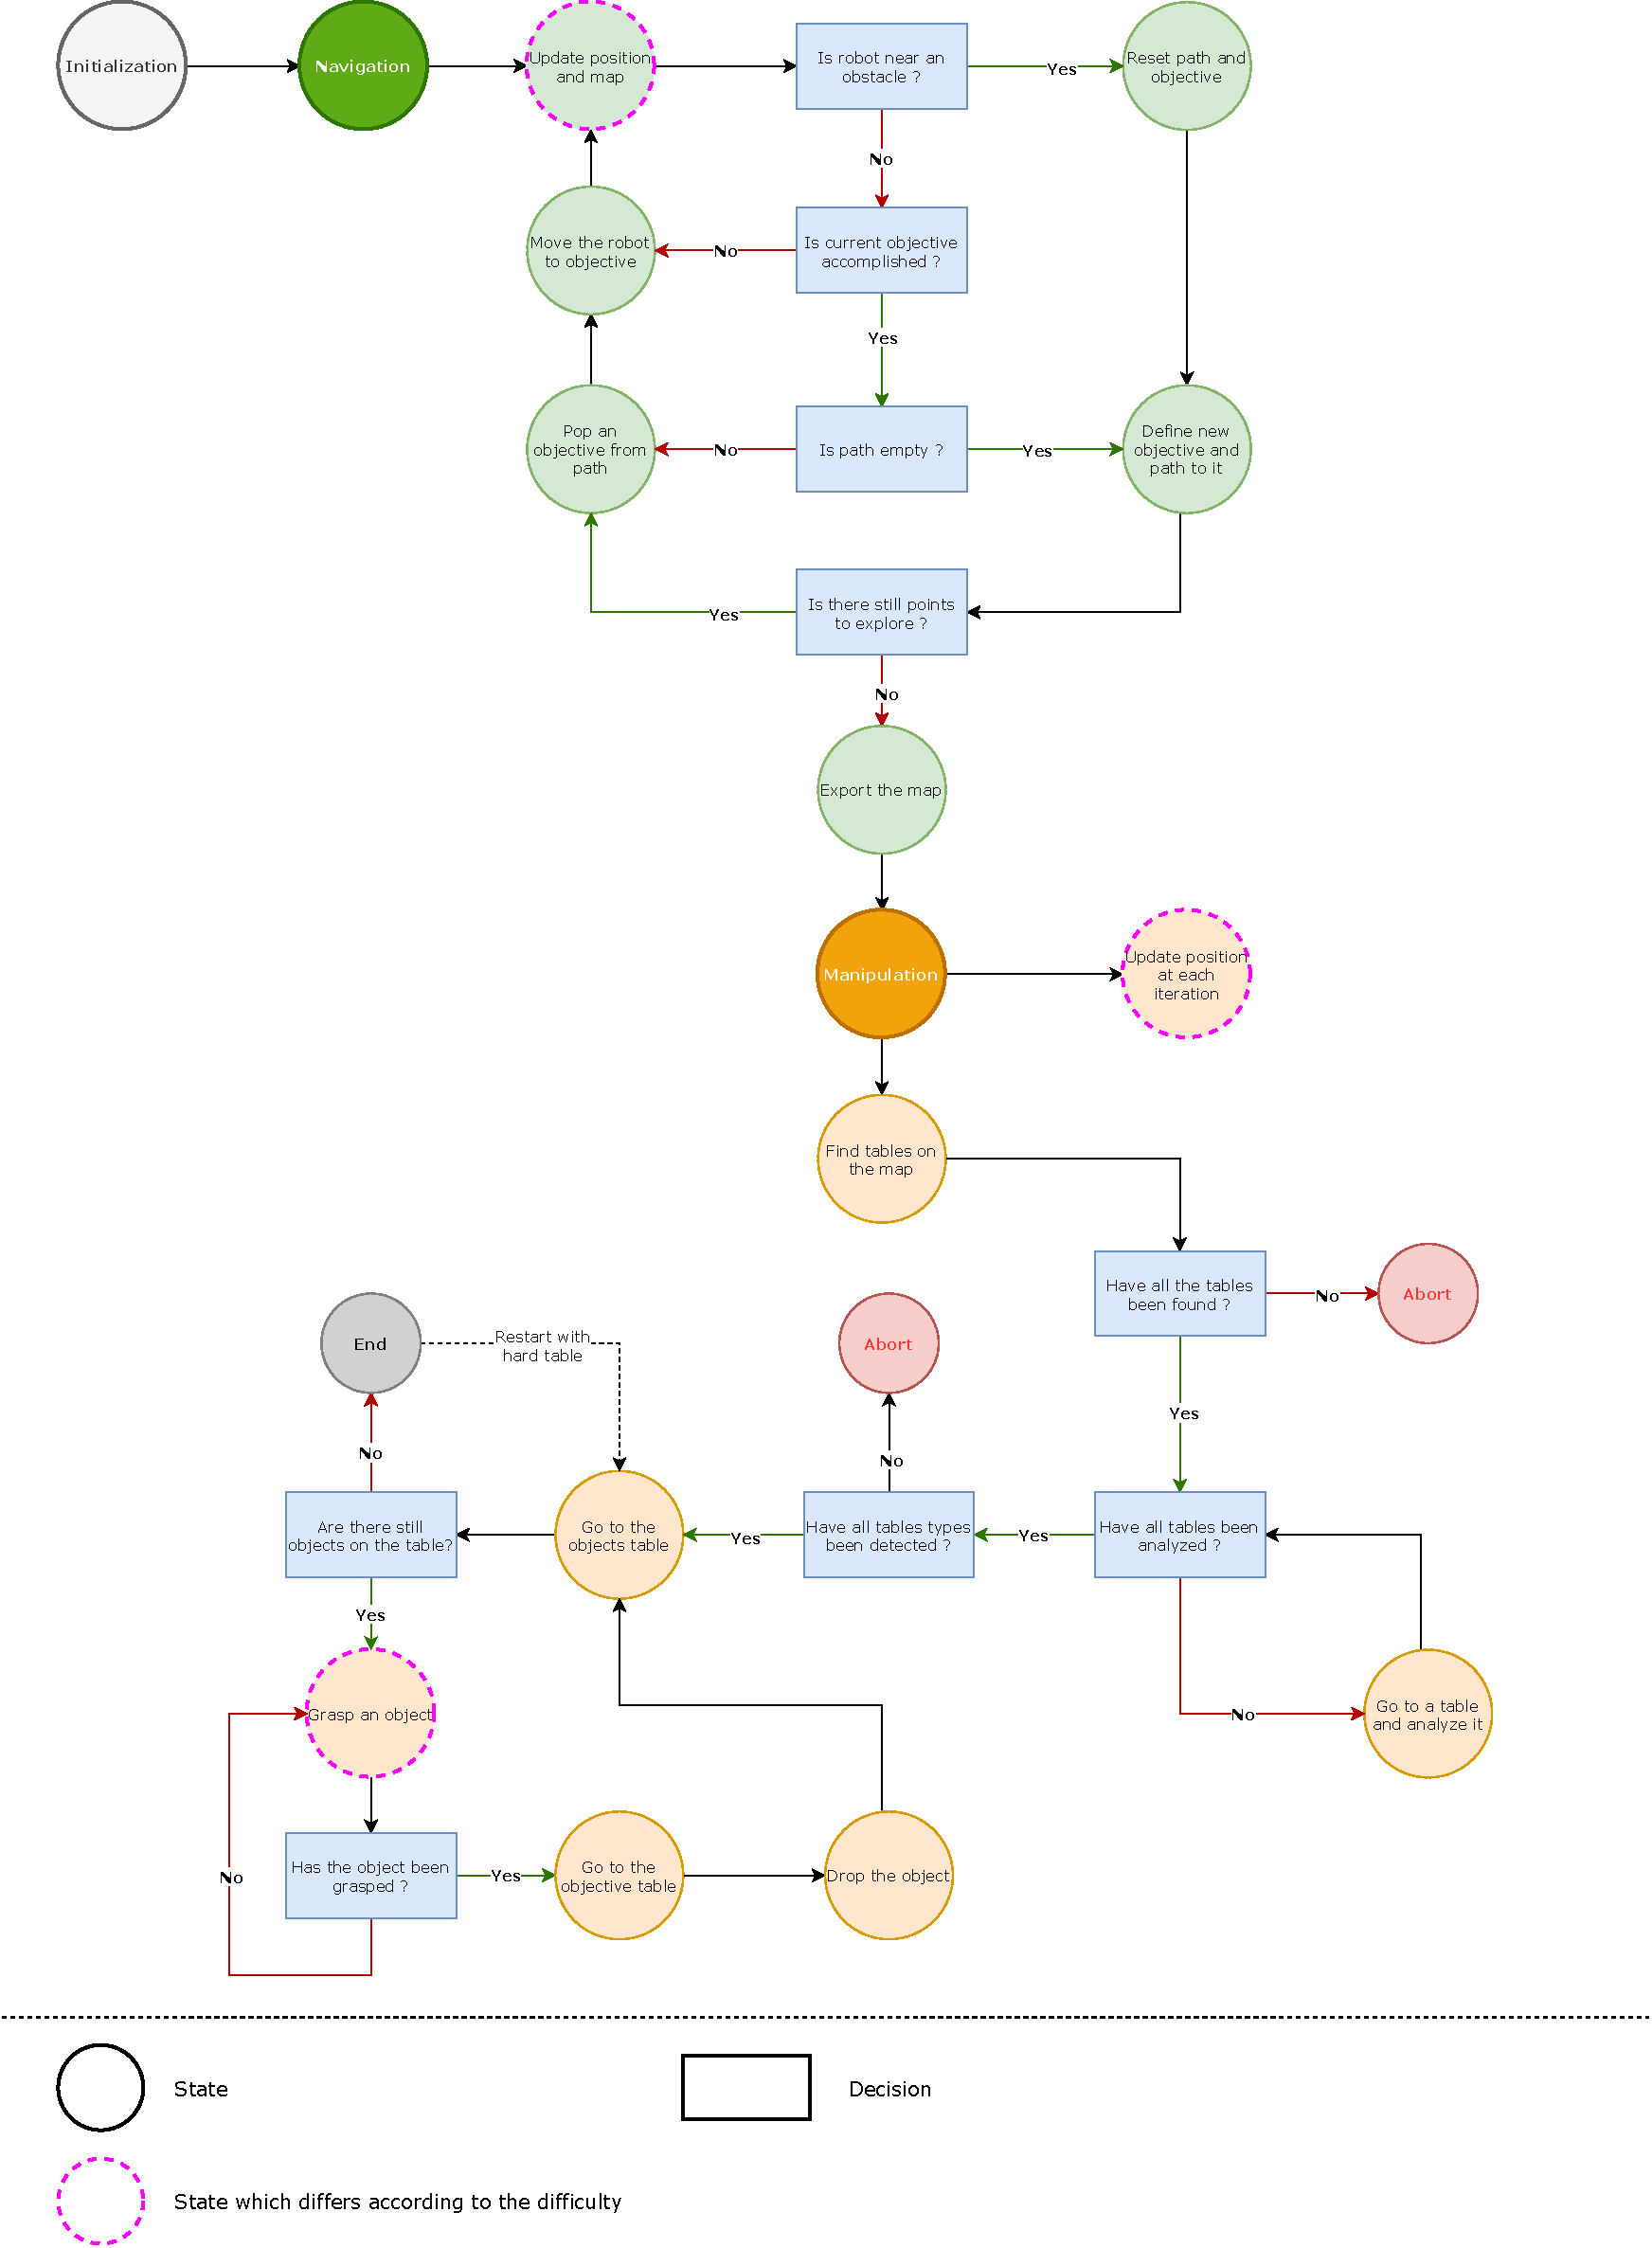
\includegraphics[width=0.9\textwidth]{resources/pdf/fsm.pdf}
        \caption{Complete finite state machine of the youBot.}
        \label{fig:fsm}
    \end{figure*}
\end{document}
